\documentclass{article}

\usepackage{fullpage}
\usepackage{url}
\usepackage{bbm}
\usepackage{graphicx}
\usepackage{amsmath}
\usepackage{physics}
\usepackage{mathtools}
\usepackage{bbold}
\usepackage{slashed}
\usepackage{pxfonts}
\usepackage{multicol}
\usepackage{mathptmx}
\usepackage{simplewick}
\usepackage{placeins}
\usepackage{booktabs}
\usepackage{tikz}
\usepackage[compat=1.1.0]{tikz-feynman}

\usepackage{lmodern}
\usepackage[T1]{fontenc}
\usepackage[fontsize=13.5pt]{fontsize}

\DeclareMathOperator{\erfi}{erfi}
\newcommand{\R}{\ensuremath{\mathbb{R}}}
\newcommand{\C}{\ensuremath{\mathbb{C}}}

\tikzset{
  counterterm/.style={
    circle,
    draw,
    inner sep=1pt,
    minimum size=3mm,
    path picture={
      \draw[black] 
      (path picture bounding box.south west) -- (path picture bounding box.north east)
      (path picture bounding box.south east) -- (path picture bounding box.north west);
    }
  }
}

\title{QFT1 Formulas}
\author{Idan Stark}

\begin{document}
\maketitle

\section{A theory of two scalars in $2+1$ dimensions}
\subsection{The Global symmetry}
The action given has two $\mathbb{Z}_2$ symmetries, one for each field:
\begin{equation}
    \phi_i \rightarrow -\phi_i
\end{equation}
This symmetry does not allow the mixing of fields, since:
\begin{equation}
\begin{gathered}
    \langle \phi_1 \phi_2 \rangle =
    \int \mathcal{D}\phi_1\mathcal{D}\phi_2 \phi_1 \phi_2 e^{iS[\phi_1, \phi_2]} = \\ =
    \int \mathcal{D}\phi_1\mathcal{D}\phi_2 \phi_1 \phi_2 e^{iS[-\phi_1, \phi_2]} =
    \int \mathcal{D}\phi_1\mathcal{D}\phi_2 (-\phi_1) \phi_2 e^{iS[\phi_1, \phi_2]} = \\ =
    -\langle \phi_1 \phi_2 \rangle
\end{gathered}
\end{equation}
\subsection{Renormalizability and counter terms}
\subsubsection*{Renormalizability}
We look for processes with positive superficial degree of divergence. In $d = 3$, and $n = 6$:
\begin{equation}
    D = d + V\left(n \frac{d-2}{2} - d\right) - N \frac{d-2}{2} = 3 - \frac{N}{2}
\end{equation}
Where $N$ is the number of external legs. Now, from the symmetry, there are three possible values for $N$ for which $D \ge 0$: $N = 2, 4, 6$, where $D > 0$ for $N = 2,4$ and $D = 0$ for $N = 6$.
\subsubsection*{Counter terms}
To see the counter-terms, we need to take the most general form of the Lagrangian. This includes all terms that preserve the symmetry, with maximal power of $\phi^6$. This gives:
\begin{equation}
    \mathcal{L} = \sum_i \left[\frac{1}{2}\left(\partial_\mu\phi_i\right)^2 + \frac{1}{2}m_i^2\phi_i^2 + g_{4i}\phi_i^4 + g_{6i}\phi_i^6\right] + \lambda_{22}\phi_1^2\phi_2^2 + \lambda_{42}\phi_1^4\phi_2^2 + \lambda_{24}\phi_1^2\phi_2^4
\end{equation}
Where we renamed $\lambda_{24} = -\frac{\lambda}{2!4!}$ for consistency. This means there is a total of eleven counter terms: for each field, there are $\delta_{Z_i}, \delta_{m_i}, \delta_{4_i}, \delta_{6_i}$, and additional three for field-field interactions $\delta_{g_{22}}, \delta_{g_{42}}, \delta_{g_{24}}$.
\subsection{$2\rightarrow2$ scattering}
\subsubsection{Possible scatterings}
As we saw in the (a), any correlation function that includes an odd number of any field will vanish. Processes that change the total mass of the system are also not allowed, since from the center of mass frame this violates conservation of four momentum, and thus breaks the Loretnz symmetry. This leaves the processes:
\begin{equation}
    \phi_1\phi_1 \rightarrow \phi_1\phi_1 \qquad
    \phi_1\phi_2 \rightarrow \phi_1\phi_2 \qquad
    \phi_2\phi_2 \rightarrow \phi_2\phi_2 \qquad
\end{equation}
\subsubsection{Processes that are not zero at leading order}
At leading order in perturbation theory, the only interaction allowed is the single vertex diagrams from $\phi_1^2\phi_2^4$. All other interactions, including counter terms, are in higher order in perturbation theory. This means that the $\phi_1\phi_1 \rightarrow \phi_1\phi_1$ cannot happen at this order, but the other two can:
\begin{center}
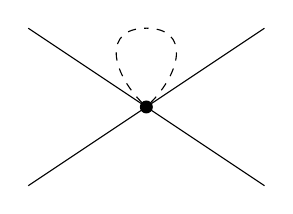
\begin{tikzpicture}[baseline=(current bounding box.center)]
  \begin{feynman}
    \vertex[dot] (v) at (0,0) {};
    \vertex (v0) at (0,1);
    \vertex (i1) at (-1.5, -1);
    \vertex (i2) at (-1.5, 1);
    \vertex (f1) at (1.5, 1);
    \vertex (f2) at (1.5, -1);
    \draw[plain] (i1) -- (v);
    \draw[plain] (i2) -- (v);
    \draw[plain] (v) -- (f1);
    \draw[plain] (v) -- (f2);
    \draw[scalar] (v) to[out=45, in=0, looseness=1.5] (v0);
    \draw[scalar] (v) to[out=135, in=180, looseness=1.5] (v0);
  \end{feynman}
\end{tikzpicture}
\hspace{3cm}
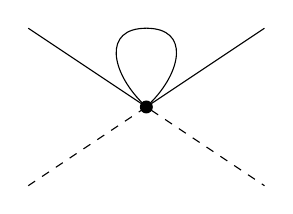
\begin{tikzpicture}[baseline=(current bounding box.center)]
  \begin{feynman}
    \vertex[dot] (v) at (0,0) {};
    \vertex (v0) at (0,1);
    \vertex (i1) at (-1.5, -1);
    \vertex (i2) at (-1.5, 1);
    \vertex (f1) at (1.5, 1);
    \vertex (f2) at (1.5, -1);
    \draw[scalar] (i1) -- (v);
    \draw[plain] (i2) -- (v);
    \draw[plain] (v) -- (f1);
    \draw[scalar] (v) -- (f2);
    \draw[plain] (v) to[out=45, in=0, looseness=1.5] (v0);
    \draw[plain] (v) to[out=135, in=180, looseness=1.5] (v0);
  \end{feynman}
\end{tikzpicture}
\end{center}
Let us notice that since we are in order $\lambda$, all counter terms, which are of order $\lambda^2$ and above, are not considered in this order of perturbation theory.
\subsubsection{Calculating $\phi_2\phi_2 \rightarrow \phi_2\phi_2$ with cutoff regularization}
For the $\phi_2\phi_2 \rightarrow \phi_2\phi_2$ process, we take the left diagram, and add the approriate counter terms:
\begin{equation}
    i\mathcal{M} = -i\lambda \int \frac{d^3k}{(2\pi)^3} \frac{i}{k^2 - m_1^2 + i\epsilon}
\end{equation}
Where we used the symmetry factor from $2$ from the loop, and an additional symmetry factor $4!$ from the permutation of external legs.
\newline
The degree of the integral is $\frac{d^3k}{k^2} \sim k$ which means the integral is linearly divergent.
\newline
Let us now define the maximal momenta $\Lambda$, move to Euclidean space $k^0 = ik_E^0$, and integrate to get:
\begin{equation}
\begin{gathered}
    i\mathcal{M} = i\frac{4\pi \lambda}{(2\pi)^3} \int_0^\Lambda \frac{k_E^2}{k_E^2 - m_1^2}dk_E = \\ =
    i\frac{4\pi \lambda}{(2\pi)^3} \left[\Lambda - m_1\text{atanh}\left(\frac{\Lambda}{m_1}\right)\right] = \\ =
    i\frac{4\pi \lambda}{(2\pi)^3} \left[\Lambda + \frac{m_1}{2}\ln(\frac{m_1 + \Lambda}{m_1 - \Lambda})\right] = \\ =
    i\frac{\lambda}{2\pi^2} \left[\Lambda + \frac{m_1}{2}\ln(\frac{m_1 + \Lambda}{m_1 - \Lambda})\right]
\end{gathered}
\end{equation}
This diverges linearly, as expected.
\subsubsection{Calculating $\phi_2\phi_2 \rightarrow \phi_2\phi_2$ with dimensional regularization}
Starting from the same linearly-diverging integral:
\begin{equation}
    i\mathcal{M} = -i\lambda \int \frac{d^3k}{(2\pi)^3} \frac{i}{k^2 - m_1^2 + i\epsilon}
\end{equation}
Changing the dimension of the momentum integral $3 \rightarrow d$
\begin{equation}
    i\mathcal{M} = -i\lambda \int \frac{d^dk}{(2\pi)^d} \frac{i}{k^2 - m_1^2 + i\epsilon}
\end{equation}
We can already use the known integral:
\begin{equation}
    \int \frac{d^dk}{(2\pi)^d} \frac{i}{k^2 - m_1^2 + i\epsilon} = -\int \frac{dk_E^d}{(2\pi)^d} \frac{1}{(k_E^2 - \Delta)^n}
    \qquad n = 1, \ \Delta = m_1^2
\end{equation}
Which gives:
\begin{equation}
    i\mathcal{M} = i\lambda \frac{1}{(4\pi)^{d/2}}\frac{\Gamma\left(1 - \frac{d}{2}\right)}{\Gamma(1)} \Delta^{\frac{d}{2} - 1}
\end{equation}
Setting $d = 3 - \epsilon$:
\begin{equation}
    i\mathcal{M} = i\lambda \frac{1}{(4\pi)^{(3 - \epsilon)/2}}\frac{\Gamma\left(\epsilon-\frac{1}{2}\right)}{\Gamma(1)} \Delta^{\frac{1}{2} - \frac{\epsilon}{2}}
\end{equation}
And taking $\epsilon \rightarrow 0$:
\begin{equation}
    i\mathcal{M} = -i\frac{1}{2\pi}\lambda m_1
\end{equation}
Using the renormalization condition
TODO: continue if I have time (if it's here it means I didn't)
\subsection{Renormalization of $\lambda$}
\subsubsection{In first order of $\lambda$}
At first order, this is simply equal to the vertex:
\begin{equation}
    \mathcal{M} = -\lambda
\end{equation}
\subsubsection{Diagrams contributing in second order of $\lambda$}
At second order, we look for diagrams that have two vertices. This immidiately gives the two loop diagram (call it the candy diagram):
\begin{center}
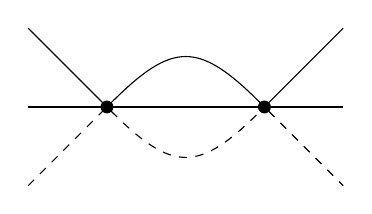
\begin{tikzpicture}[baseline=(current bounding box.center)]
  \begin{feynman}
    \vertex[dot] (v1) at (-1,0) {};
    \vertex[dot] (v2) at (1,0) {};
    \vertex (i1) at (-2, -1);
    \vertex (i2) at (-2, 0);
    \vertex (i3) at (-2, 1);
    \vertex (f1) at (2, 1);
    \vertex (f2) at (2, 0);
    \vertex (f3) at (2, -1);
    \draw[scalar] (i1) -- (v1);
    \draw[plain] (i2) -- (v1);
    \draw[plain] (i3) -- (v1);
    \draw[plain] (v2) -- (f1);
    \draw[plain] (v2) -- (f2);
    \draw[scalar] (v2) -- (f3);
    \draw[plain] (v1) to[out=45, in=135, looseness=1.5] (v2);
    \draw[plain] (v1) to[out=0, in=180, looseness=1.5] (v2);
    \draw[scalar] (v1) to[out=-45, in=-135, looseness=1.5] (v2);
  \end{feynman}
\end{tikzpicture}
\end{center}
There are additionally two diagrams: the matching T and U channels, which can be viewed simply permutations over the external legs.
\subsubsection{The Scattering amplitude}
We can write the scattering using the Feynman rules:
\begin{equation}
\begin{gathered}
    i\mathcal{M} = i\frac{\lambda^2}{2}\int \frac{d^3q_1}{(2\pi)^3} \frac{d^3q_2}{(2\pi)^3}\frac{i}{q_1^2-m_1^2+i\epsilon}\frac{i}{q_2^2-m_1^2+i\epsilon}\frac{i}{(p_1 + p_2 + p_3 - q_1 - q_2)^2-m_1^2+i\epsilon} + \\ +
    (p_2 \rightarrow - p_5) +
    (p_2 \rightarrow - p_6) +
    (p_3 \rightarrow - p_5) +
    (p_3 \rightarrow - p_6) +
    (p_2 + p_3 \rightarrow -p_5 - p_6)
\end{gathered}
\end{equation}
This integral acts like $\frac{d^6q}{q^6} \sim 1$, which means it will diverge logarithmically, as expected from our previous computations.
\subsection{The beta function for high energy scales}
We work at energy scale $M^2 \gg m_i^2$, so let us set $m_i = 0$ to get (for the first diagram):
\begin{equation}
    i\frac{\lambda^2}{2}\int \frac{d^3q_1}{(2\pi)^3} \frac{d^3q_2}{(2\pi)^3}\frac{i}{q_1^2+i\epsilon}\frac{i}{q_2^2+i\epsilon}\frac{i}{(p_1 + p_2 + p_3 - q_1 - q_2)^2+i\epsilon}
\end{equation}
Starting from the integral over $q_2$, which converges, by performing Feynman's trick:
\begin{equation}
\begin{gathered}
    \int \frac{d^3q_1}{(2\pi)^3} \frac{d^3q_2}{(2\pi)^3}\frac{i}{q_1^2+i\epsilon}\frac{i}{q_2^2+i\epsilon}\frac{i}{(p_1 + p_2 + p_3 - q_1 - q_2)^2+i\epsilon} = \\ =
    -2i\int \frac{d^3q_1}{(2\pi)^3} \frac{d^3q_2}{(2\pi)^3}\int_0^1dx\int_0^{1-x}dy \frac{1}{[x(p_1 + p_2 + p_3 - q_1 - q_2)^2 + yq_1^2 + zq_2^2]^3}
\end{gathered}
\end{equation}
\newpage
\section{Scattering in the Abelian Higgs model}
\subsection{Scattering amplitude dependence on gauge}
The scattering amplitude is a physical quantity. As such, it must be gauge independent.
\subsection{The limit $\xi \rightarrow \infty$}
In this limit, we can ignore $\phi$ and are left with a single interaction vertex between the $h$ field and the photon:
\begin{equation}
    \mathcal{L}_1 = \frac{e^2}{2}h^2A_\mu^2
\end{equation}
This means, that up to order $e^2$, the only contributing diagrasm to the $hh\rightarrow\gamma\gamma$ scattering are the single vertex diagram:
\newline
I'm writing this right after you told us to finish. I just now found the term $e^2vA_\mu^2 h$ that allows for an internal photon propegator, and thus adds the s, t, and u channels that are missing here.
\begin{center}
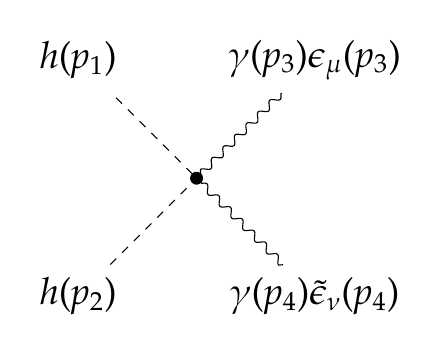
\begin{tikzpicture}[baseline=(current bounding box.center)]
  \begin{feynman}
    \vertex[dot] (v1) at (0,0) {};
    \vertex (i1) at (-1.5, -1.5) {$h(p_2)$};
    \vertex (i2) at (-1.5, 1.5) {$h(p_1)$};
    \vertex (f1) at (1.5, 1.5) {$\gamma(p_3)\epsilon_\mu(p_3)$};
    \vertex (f2) at (1.5, -1.5) {$\gamma(p_4)\tilde{\epsilon}_\nu(p_4)$};
    \draw[scalar] (i1) -- (v1);
    \draw[scalar] (v1) -- (i2);
    \draw[photon] (f1) -- (v1);
    \draw[photon] (v1) -- (f2);
  \end{feynman}
\end{tikzpicture}
\end{center}
While topologically they are the same, each diagram has distinct photon index contraction. They do not have any loops of undetermined momenta, so they simply give the value of the vertex. Of course, the exchange of scalar momenta doesn't change anything, and is absorbed by the symmetry factor:
\begin{equation}
    i\mathcal{M} = -ie^2\eta^{\mu\nu}\left[
        \epsilon_\mu(p_3)\tilde{\epsilon}_\nu(p_4)
        + \epsilon_\nu(p_3)\tilde{\epsilon}_\mu(p_4)
    \right]
\end{equation}
\begin{equation}
    i\mathcal{M} = -i4e^2\epsilon_\mu(p_3)\tilde{\epsilon}^\mu(p_4)
\end{equation}
\subsection{The limit $\xi = 0$}
In this limit, in addition to the vertex from the previous section, there is an additional vertex:
\begin{equation}
    \mathcal{L}_2 = -e\left[\phi \partial_\mu h - h \partial_\mu\phi\right]A^\mu
\end{equation}
This allowed for additional 2 vertex diagrams, specifically the t and s channels, to contribute to the scattering:
\begin{center}
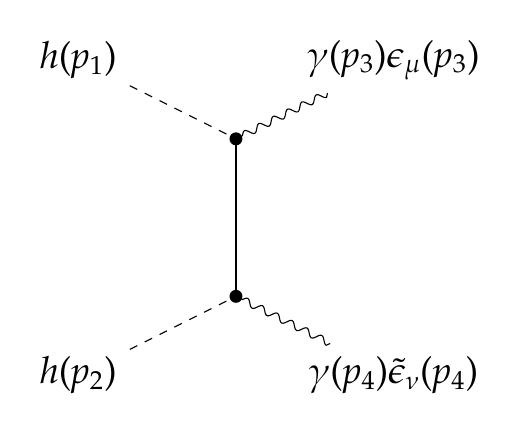
\begin{tikzpicture}[baseline=(current bounding box.center)]
  \begin{feynman}
    \vertex[dot] (v1) at (0,-1) {};
    \vertex[dot] (v2) at (0,1) {};
    \vertex (i1) at (-2, -2) {$h(p_2)$};
    \vertex (i2) at (-2, 2) {$h(p_1)$};
    \vertex (f1) at (2, 2) {$\gamma(p_3)\epsilon_\mu(p_3)$};
    \vertex (f2) at (2, -2) {$\gamma(p_4)\tilde{\epsilon}_\nu(p_4)$};
    \draw[scalar] (i1) -- (v1);
    \draw[scalar] (i2) -- (v2);
    \draw[photon] (v1) -- (f2);
    \draw[photon] (v2) -- (f1);
    \draw[plain] (v1) -- (v2);
  \end{feynman}
\end{tikzpicture}
\hspace{0.5cm}
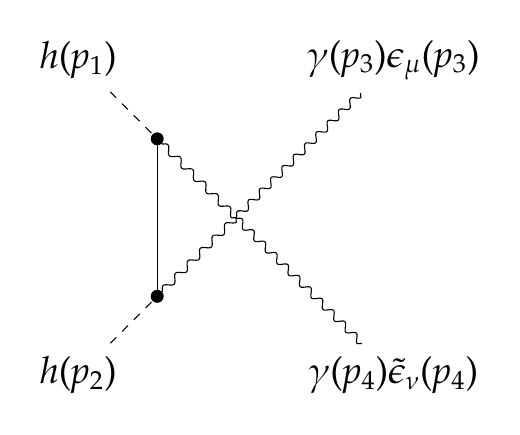
\begin{tikzpicture}[baseline=(current bounding box.center)]
  \begin{feynman}
    \vertex (i1) at (-2, -2) {$h(p_2)$};
    \vertex (i2) at (-2, 2) {$h(p_1)$};
    \vertex (f1) at (2, 2) {$\gamma(p_3)\epsilon_\mu(p_3)$};
    \vertex (f2) at (2, -2) {$\gamma(p_4)\tilde{\epsilon}_\nu(p_4)$};
    \vertex[dot] (v1) at (-1, 1) {};
    \vertex[dot] (v2) at (-1, -1) {};
    \vertex (v0) at (0,0);
    \draw[scalar] (i2) -- (v1);
    \draw[scalar] (i1) -- (v2);
    \draw[photon] (v0) -- (f1);
    \draw[photon] (v0) -- (f2);
    \draw[photon] (v2) -- (v0);
    \draw[photon] (v1) -- (v0);
    \draw[plain] (v2) -- (v1);
  \end{feynman}
\end{tikzpicture}
\end{center}
This gives:
\begin{equation}
\begin{gathered}
    i\mathcal{M} = \frac{(-ie)^2}{2}\left[p_1 - (p_3 - p_1)\right]^\mu\frac{i}{(p_3 - p_1)^2}\left[p_2 - (p_4 - p_2)\right]^\nu\epsilon_\mu(p_3)\tilde{\epsilon}_\nu(p_4) + \\ +
    \frac{(-ie)^2}{2}\left[p_2 - (p_3 - p_2)\right]^\mu\frac{i}{(p_4 - p_1)^2}\left[p_1 - (p_4 - p_1)\right]^\nu\epsilon_\mu(p_3)\tilde{\epsilon}_\nu(p_4) = \\ =
    -i2e^2\left[
        \frac{p_1^\mu p_2^\nu}{(p_3 - p_1)^2} +
        \frac{p_2^\mu p_1^\nu}{(p_4 - p_1)^2}
    \right]\epsilon_\mu(p_3)\tilde{\epsilon}_\nu(p_4)
\end{gathered}
\end{equation}
Where we used $p_i\cdot\epsilon(p_i) = 0$. Changing the indices in the second fractions gives:
\begin{equation}
\begin{gathered}
    i\mathcal{M} = 
    -i2e^2p_1^\mu p_2^\nu\left[
        \frac{\epsilon_\mu(p_3)\tilde{\epsilon}_\nu(p_4)}{(p_3 - p_1)^2} +
        \frac{\epsilon_\nu(p_3)\tilde{\epsilon}_\mu(p_4)}{(p_4 - p_1)^2}
    \right]
\end{gathered}
\end{equation}
\subsection{Comparing the two}
The two results from the two gauges are quite different. This is because of the error I have explained at the beginning of the answer. 
\newpage
\section{"Integrating out" a massive particle}
\subsection{Calculating the integral}
The path integral is:
\begin{equation}
    Z = \int \mathcal{D}\chi\mathcal{D}\psi e^{iS[\chi,\psi]}
\end{equation}
We can now seperate the action into action that is dependent on $\chi$ and action that is not (it's marked $S_i$, but I know it's not only interactions):
\begin{equation}
    S = S_0[\psi] + S_i[\chi,\psi]
\end{equation}
And then the integral becomes:
\begin{equation}
    Z = \int \mathcal{D}\psi e^{iS_0[\psi]} \int \mathcal{D}\chi e^{iS_i[\psi, \chi]}
\end{equation}
Now we can perform the second integral. Writing $S_i$ explicitly:
\begin{equation}
    S_i = \int d^4x \left[
        \frac{1}{2}\left(\partial_\mu\chi\right) - \frac{1}{2}M^2\chi^2 - g\bar{\psi}\psi\chi
    \right]
\end{equation}
So, we can define the source:
\begin{equation}
    J(x) = g\bar{\psi}(x)\psi(x)
\end{equation}
To get (using the hint):
\begin{equation}
\begin{gathered}
    Z_i = \int \mathcal{D}\chi e^{iS_i[\psi, \chi]} = \\ = Z[0]\exp(-\frac{g^2}{2}\int d^4x d^4y \bar{\psi}(x)\psi(x) \Delta_F(x - y)\bar{\psi}(y)\psi(y))
\end{gathered}
\end{equation}
Where $\Delta_F$ is the Feynman propegator. So, our effective action can be written as:
\begin{equation}
    S = S_0[\psi] - \frac{g^2}{2}\int d^4x d^4y \bar{\psi}(x)\psi(x) \Delta_F(x - y)\bar{\psi}(y)\psi(y)
\end{equation}
Expanding the fields that are y-dependent:
\begin{equation}
\begin{gathered}
    S = S_0[\tilde{\psi}] - \frac{g^2}{2}\int d^4x d^4y\bar{\psi}(x)\psi(x) \times \\ \times \int \frac{d^4k}{(4\pi)^4}\frac{d^4p}{(4\pi)^4} e^{-iky} \frac{ie^{-ip(x - y)}}{p^2 - M^2 + i\epsilon}\bar{\psi}(k)\psi(k)
\end{gathered}
\end{equation}
From the y integral, we get a delta function $\delta^{(4)(p-k)}$, and we can use it to solve the k integral:
\begin{equation}
\begin{gathered}
    S = S_0[\tilde{\psi}] - \frac{g^2}{2}\int d^4x\bar{\psi}(x)\psi(x) \int \frac{d^4p}{(4\pi)^4} \frac{ie^{-ipx}}{p^2 - M^2 + i\epsilon}\bar{\psi}(p)\psi(p)
\end{gathered}
\end{equation}
Now, let us inverse the Fourier transform from the integral of $p$. We can do that if we first remove $i\epsilon$ and take the Taylor expansion:
\begin{equation}
    \frac{i}{p^2 - M^2 + i\epsilon} = -i \sum_0^\infty \frac{p^{2n}}{M^{2n+2}}
\end{equation}
To get:
\begin{equation}
\begin{gathered}
    \int \frac{d^4p}{(4\pi)^4} \frac{ie^{-ipx}}{p^2 - M^2 + i\epsilon}\bar{\psi}(p)\psi(p) = i\sum_{n=0}^\infty \frac{1}{M^{2n+2}} \int \frac{d^4p}{(4\pi)^4} e^{-ipx} p^{2n}\bar{\psi}(p)\psi(p) = \\ =
    i\sum_{n=0}^\infty \frac{1}{M^{2n+2}} \left(\partial_\mu\partial^\mu\right)^n \bar{\psi}(x)\psi(x)
\end{gathered}
\end{equation}
Which gives the final result:
\begin{equation}
    S_{eff} = \bar{\psi}(i\slashed{\partial} - m)\psi - i\frac{g^2}{2}\sum_{n=0}^\infty \frac{1}{M^{2n+2}} \int d^4x \bar{\psi}(x)\psi(x)\left(\partial_\mu\partial^\mu\right)^n\bar{\psi}(x)\psi(x)
\end{equation}
Im sure this can be simplified further, I just don't have the time.
\subsection{Measuring it}
A simple way to measure this would be to take the $\bar{\psi}\psi \rightarrow \bar{\psi}\psi$ scattering amplitude at different momenta, but similar energy scales. This will allow to take the percieved bare coupling of the interaction as a function of the momentum $g(k)$. Then, compare it to the propegator the coefficient written in the action (after regularization and renormalization).
\end{document}